\documentclass[theme=workflow,aspectratio=169,fontset=tech]{Hypo-Slide}

\usepackage{graphicx}
\usepackage{booktabs}
\usepackage{tabularx}
\usepackage{array}
\usepackage{multicol}
\usepackage{tikz}
\usepackage{pgfplots}
\usepackage{adjustbox}
\usetikzlibrary{arrows.meta,positioning,fit,matrix,trees,calc}
\pgfplotsset{compat=1.18}
\graphicspath{{assets/}{figures/}{vendor/Hypoxanthine-LaTeX/assets/}}

\HypoSlideSetup{
  title={Hypo-Workflow},
  subtitle={从 AI Coding 使用经验到 Harness Engineering 工作流},
  author={Hypo-Workflow Project Draft},
  institute={Technical Report / Lab Presentation},
  date={2026-05-01},
  cover={assets/opencode-observability.png}
}
\author[Project Draft]{Hypo-Workflow Project Draft}

\newcommand{\WorkflowSectionFrame}[3]{
  \begin{frame}[plain]
    \begin{tikzpicture}[remember picture,overlay]
      \node[anchor=center,inner sep=0pt] at (current page.center)
        {\includegraphics[width=\paperwidth,height=\paperheight]{#3}};
      \fill[white,opacity=0.88] (current page.north west) rectangle ([xshift=0.54\paperwidth]current page.south west);
      \fill[WorkflowBlue!80] ([xshift=0.055\paperwidth,yshift=-0.18\paperheight]current page.north west) rectangle ++(0.008\paperwidth,-0.28\paperheight);
    \end{tikzpicture}
    \vspace*{1.25cm}
    \hspace*{0.95cm}
    \begin{minipage}{0.42\paperwidth}
      {\Large\bfseries\color{WorkflowBlue}#1\par}
      \vspace{0.55cm}
      {\fontsize{21}{25}\selectfont\bfseries\color{WorkflowText}#2\par}
    \end{minipage}
  \end{frame}
}

\newcommand{\WorkflowFigureFrame}[3]{
  \begin{frame}{#1}
    \centering
    \adjustbox{max width=0.92\linewidth,max totalheight=0.64\textheight,center}{\input{#2}}
    \vspace{0.3cm}

    {\small\color{WorkflowMuted}#3}
  \end{frame}
}

\newcommand{\CommandRow}[3]{\texttt{#1} & #2 & #3 \\}

\AtBeginSection[]{
  \begin{frame}{报告结构}
    \small
    \tableofcontents[currentsection,hideothersubsections]
  \end{frame}
}

\begin{document}

\begin{frame}[plain]
  \titlepage
\end{frame}

\begin{frame}{报告结构}
  \tableofcontents
\end{frame}

\section{动机与问题}
\WorkflowSectionFrame{Part I}{七段使用路径如何逼出工作流}{assets/opencode-observability.png}

\begin{frame}{路径 1：网页模型与 Cherry Studio}
  \begin{columns}[T,totalwidth=\textwidth]
    \column{0.56\textwidth}
    \begin{block}{工具状态}
      Web GPT、Gemini、Cherry Studio + DeepSeek 解决的是“先能问、先能写、先能改”的问题。
    \end{block}
    \begin{itemize}
      \item 优点：进入成本低，适合探索想法和单点解释。
      \item 缺口：不能稳定理解完整 repo，也不能把项目约束长期留住。
      \item 结果：用户必须把代码、上下文、规范、当前目标反复搬进聊天窗口。
    \end{itemize}
    \column{0.38\textwidth}
    \begin{alertblock}{后来留下的需求}
      AI Coding 不能只依赖一次对话的聪明程度；它需要一个能保存上下文、状态和规则的外部轨道。
    \end{alertblock}
  \end{columns}
\end{frame}

\begin{frame}{路径 2：Copilot 与 Hypo-LaTeX}
  \begin{columns}[T,totalwidth=\textwidth]
    \column{0.54\textwidth}
    \begin{block}{真实场景}
      做 Hypo-LaTeX 时，Copilot 可以补全局部代码，但每次写 \texttt{CHANGELOG}、整理 Git、按规范发布，都要手工贴一长串 Prompt。
    \end{block}
    \begin{itemize}
      \item 它擅长“下一行”，不擅长“这个项目现在处于什么阶段”。
      \item 规范不是系统的一部分，而是用户每次临时注入的材料。
      \item Copilot 连续封了三个号之后，单一工具入口的脆弱性也被放大。
    \end{itemize}
    \column{0.40\textwidth}
    \begin{exampleblock}{柳暗花明}
      被迫另寻出路反而暴露了更根本的问题：真正要建设的不是某个 Copilot 替代品，而是跨工具、可恢复、可审计的工作流。
    \end{exampleblock}
  \end{columns}
\end{frame}

\begin{frame}{路径 3：AntiGravity 与自动化幻觉}
  \begin{block}{当时吸引人的地方}
    AntiGravity 带来的感觉是“终于可以不只补全，而是让工具自己往前走”。
  \end{block}
  \begin{columns}[T,totalwidth=\textwidth]
    \column{0.31\textwidth}
    \begin{block}{推进速度}
      初期任务能很快展开，Agent 像是在主动承担工作。
    \end{block}
    \column{0.31\textwidth}
    \begin{block}{可控性}
      一旦目标变复杂，用户很难判断它到底沿着哪条假设在执行。
    \end{block}
    \column{0.31\textwidth}
    \begin{block}{验证}
      自动化如果没有测试、日志和中间状态，速度本身会变成风险。
    \end{block}
  \end{columns}
  \vspace{0.25cm}
  \begin{alertblock}{后来留下的需求}
    自动执行必须和可见计划、可回滚状态、可重复验证绑在一起。
  \end{alertblock}
\end{frame}

\begin{frame}{路径 4：Claude Code 与 Bill}
  \begin{columns}[T,totalwidth=\textwidth]
    \column{0.50\textwidth}
    \begin{block}{Bill 的前半段}
      刚开始搭建时，Claude 的一次性实现能力很强，界面、数据结构、交互雏形都能快速出来。
    \end{block}
    \begin{block}{Bill 的后半段}
      UI 显示问题开始反复出现：改一次看似修好，下一轮又把别处带坏。
    \end{block}
    \column{0.44\textwidth}
    \begin{alertblock}{痛点}
      它不主动补文档，也不会自然形成可验收的视觉证据。用户说一句，它干半天，最后发现很多是假设错了之后的忙碌。
    \end{alertblock}
  \end{columns}
\end{frame}

\begin{frame}{路径 5：Superpowers 与 Agent}
  \begin{columns}[T,totalwidth=\textwidth]
    \column{0.48\textwidth}
    \begin{exampleblock}{为什么前期很好用}
      Claude + Superpowers 已经有早期 Harness 的形态：能讨论、能落盘、能把一部分行为变成可复用流程。
    \end{exampleblock}
    \column{0.48\textwidth}
    \begin{alertblock}{为什么后期不够}
      到 Agent 项目进入修 Bug 和加功能阶段，Superpowers 缺少全局观。每次改动都像局部补丁，为了改而改，改一个地方引入一串新问题。
    \end{alertblock}
  \end{columns}
  \vspace{0.35cm}
  \begin{block}{定位}
    Superpowers 不是失败品，而是早期 Harness：它证明“外部约束层”有用，也暴露出这层必须更系统化。
  \end{block}
\end{frame}

\begin{frame}{路径 6：Notion AI + Codex 与 Research / Info}
  \begin{columns}[T,totalwidth=\textwidth]
    \column{0.50\textwidth}
    \begin{block}{工作方式}
      Notion AI 负责整理文档和生成 Prompt，Codex 负责执行，Research / Info 这类项目开始形成“规划文档 + 实现 Agent”的分工。
    \end{block}
    \begin{itemize}
      \item 规划更清楚了。
      \item 执行更工程化了。
      \item 但两者之间仍然靠人复制粘贴。
    \end{itemize}
    \column{0.44\textwidth}
    \begin{alertblock}{关键发现}
      当用户只是在 Notion 和 Codex 之间搬运 Prompt 时，本质上已经在手工扮演 workflow runtime。
    \end{alertblock}
  \end{columns}
\end{frame}

\begin{frame}{路径 7：Hypo-Workflow 成形}
  \begin{block}{转折点}
    这些经历最后汇成同一个判断：与其不断换更聪明的对话入口，不如把计划、状态、规则、验证、恢复和报告做成项目的一部分。
  \end{block}
  \begin{columns}[T,totalwidth=\textwidth]
    \column{0.31\textwidth}
    \begin{block}{文件}
      \texttt{.pipeline/} 成为事实源，不再依赖聊天记忆。
    \end{block}
    \column{0.31\textwidth}
    \begin{block}{命令}
      \texttt{/hw:*} 把常见工作流入口固化下来。
    \end{block}
    \column{0.31\textwidth}
    \begin{block}{验证}
      tests、reports、progress、logs 共同构成可审计闭环。
    \end{block}
  \end{columns}
\end{frame}

\begin{frame}{为什么“多写一点 Prompt”仍然不够}
  \begin{block}{核心判断}
    Prompt 可以补救一次，但不能稳定替代状态系统、计划系统和验证系统。
  \end{block}
  \begin{itemize}
    \item 上下文窗口天然是局部的，不能天然等价于项目记忆。
    \item 规则越依赖人工复述，越容易在疲劳、中断和换模型时丢失。
    \item 模型会在错误前提上持续自我强化，直到用户重新拉回。
    \item 中断之后如果没有文件化进度，很难恢复到同一工程状态。
  \end{itemize}
\end{frame}

\begin{frame}{六个核心约束：先看全图}
  \small
  \begin{tabularx}{\textwidth}{p{0.22\linewidth}X}
    \toprule
    约束 & 含义 \\
    \midrule
    Context management & Agent 需要知道当前代码、目标、历史决策和未完成事项，而不是只看最后几条消息。 \\
    Repeated prompt feeding & 用户不应该每次都重新粘贴风格、Git、测试、文档和验收规则。 \\
    Self-deception risk & 模型会把“我已经做了”说得很像真的，因此需要外部证据。 \\
    Style persistence & 代码风格、文档风格、交互风格必须跨会话保留。 \\
    Iteration drift & 多轮修改会逐渐偏离原问题，尤其在 UI 和 Bug 修复中明显。 \\
    Interruption / recovery & 真实开发一定会中断，所以恢复不能靠模型临场回忆。 \\
    \bottomrule
  \end{tabularx}
\end{frame}

\begin{frame}{约束 1-2：Context 与 Prompt 不是同一件事}
  \begin{columns}[T,totalwidth=\textwidth]
    \column{0.48\textwidth}
    \begin{block}{Context management}
      问题不是“窗口够不够长”，而是哪些事实应该被组织、压缩、排序、引用和更新。项目状态、队列、日志、规则都需要有稳定位置。
    \end{block}
    \column{0.48\textwidth}
    \begin{block}{Repeated prompt feeding}
      如果每次开始都要贴同一套工作规范，说明规范还没有进入系统。Hypo-Workflow 的做法是把它们变成 rules、skills、commands 和 report contracts。
    \end{block}
  \end{columns}
\end{frame}

\begin{frame}{约束 3-4：证据与风格必须外置}
  \begin{columns}[T,totalwidth=\textwidth]
    \column{0.48\textwidth}
    \begin{block}{Self-deception risk}
      Agent 很容易用完整的叙述覆盖不完整的执行。解决方式不是“更相信它”，而是要求 test output、diff、PDF、截图、log、report 这些外部证据。
    \end{block}
    \column{0.48\textwidth}
    \begin{block}{Style persistence}
      用户不应该在第十轮还提醒“别乱改 Git”“别删用户文件”“报告要中文”。稳定风格需要规则文件和 adapter，而不是口头提醒。
    \end{block}
  \end{columns}
\end{frame}

\begin{frame}{约束 5-6：长期迭代需要恢复机制}
  \begin{columns}[T,totalwidth=\textwidth]
    \column{0.48\textwidth}
    \begin{block}{Iteration drift}
      当一个 Bug 引出三个新 Bug，通常不是模型不会写代码，而是缺少目标边界、验证边界和变更审计。
    \end{block}
    \column{0.48\textwidth}
    \begin{block}{Interruption / recovery}
      中断不是异常路径，而是长期协作的常态。状态、心跳、当前步骤、未完成原因必须落在文件里，恢复才不靠猜。
    \end{block}
  \end{columns}
\end{frame}

\section{Harness Engineering}
\WorkflowSectionFrame{Part II}{把经验变成外部工程约束层}{assets/gpt-image/file-first-architecture.png}

\begin{frame}{Harness Engineering}
  \begin{definition}{定义}{def:harness}
    Harness Engineering 是围绕 AI Agent 构建外部工程约束层：把 context、plans、state、rules、evaluation、recovery 与 collaboration protocol 固化到文件和工具里。
  \end{definition}
  \vspace{0.2cm}
  \begin{itemize}
    \item 它不替模型思考，但会限制模型在哪些轨道上思考。
    \item 它不追求把 Agent 变成 runner，而是让 Agent 在可审计的项目事实源上工作。
    \item 它的目标是降低长期协作中的丢上下文、漂移、幻觉和恢复成本。
  \end{itemize}
\end{frame}

\WorkflowFigureFrame{Execution Loop}{figures/execution-loop.tex}{从 Plan 到 Report，再到 Evaluate 与 Recover，形成可重复执行的闭环}

\begin{frame}{四条机制轴}
  \begin{columns}[T,totalwidth=\textwidth]
    \column{0.48\textwidth}
    \begin{block}{Execution loop}
      Plan、Execute、Review、Report、Evaluate、Recover 不是口号，而是每个 Milestone 都要留下的证据链。
    \end{block}
    \begin{block}{Layering}
      Project、Cycle、Feature、Milestone、Patch 分别承载不同粒度，不让一个状态文件背所有语义。
    \end{block}
    \column{0.48\textwidth}
    \begin{block}{Behavior solidification}
      重复出现的提醒会沉淀成 rules、skills、commands、tests 和 templates。
    \end{block}
    \begin{block}{Automatic maintenance}
      README、Skill 分发、release、progress、logs 这些维护任务也要进入自动化约束。
    \end{block}
  \end{columns}
\end{frame}

\begin{frame}{为什么坚持 File-First}
  \begin{columns}[T,totalwidth=\textwidth]
    \column{0.48\textwidth}
    \begin{block}{聊天窗口的问题}
      \begin{itemize}
        \item 状态会漂移
        \item 历史难以索引
        \item 中断后恢复成本高
      \end{itemize}
    \end{block}
    \column{0.48\textwidth}
    \begin{block}{文件协议的收益}
      \begin{itemize}
        \item 人与 Agent 共用同一事实源
        \item 平台 adapter 可以只做投影
        \item 规划、执行、归档都可审计
      \end{itemize}
    \end{block}
  \end{columns}
\end{frame}

\WorkflowFigureFrame{\texttt{.pipeline/} File Protocol}{figures/pipeline-protocol.tex}{状态、队列、日志、指标、报告都进入统一目录协议}

\begin{frame}{File-First Architecture：架构润色版}
  \centering
  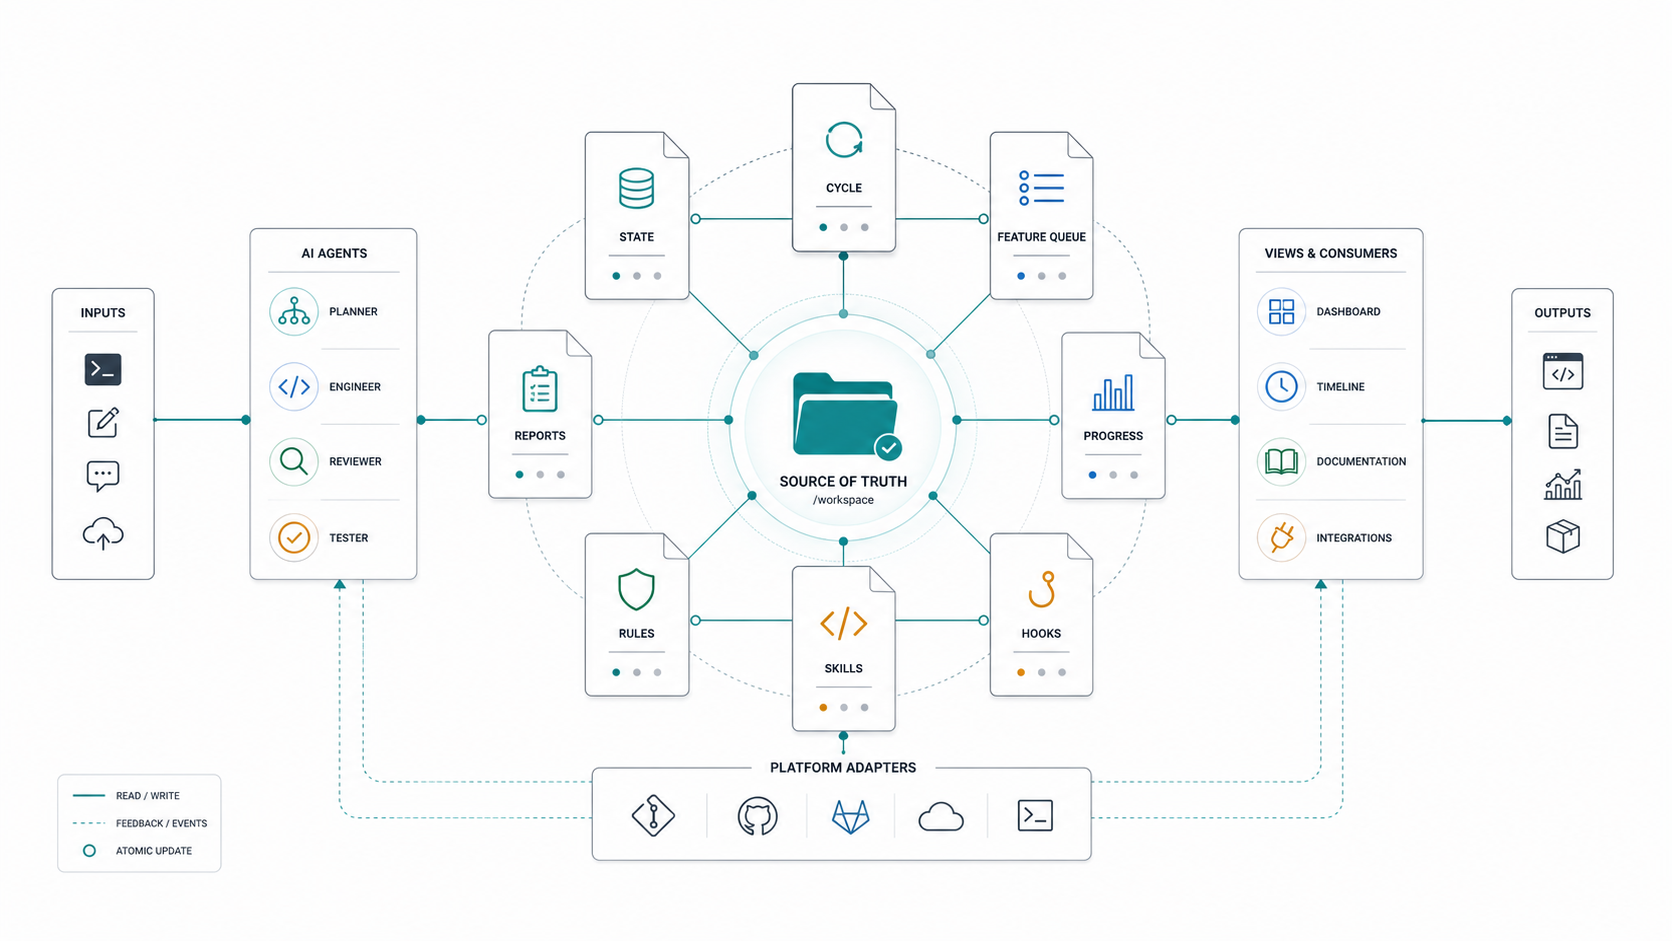
\includegraphics[width=0.86\linewidth,height=0.66\textheight,keepaspectratio]{assets/gpt-image/file-first-architecture.png}
  \vspace{0.25cm}

  {\small\color{WorkflowMuted}概念图负责帮助读者建立直觉；严格字段关系继续由 TikZ 图、真实 YAML 和测试合同作证。}
\end{frame}

\WorkflowFigureFrame{Project / Cycle / Feature / Milestone / Patch}{figures/hierarchy.tex}{Cycle 提供交付边界，Feature 提供调度层，Milestone 提供执行粒度，Patch 处理旁路修复}

\begin{frame}{失败恢复不是补充功能，而是主路径的一部分}
  \begin{columns}[T,totalwidth=\textwidth]
    \column{0.48\textwidth}
    \begin{block}{显式控制}
      \begin{itemize}
        \item \texttt{gate: confirm}
        \item skip / defer
        \item Patch 旁路
      \end{itemize}
    \end{block}
    \column{0.48\textwidth}
    \begin{block}{会话恢复}
      \begin{itemize}
        \item Stop / Resume
        \item Chat Mode
        \item heartbeat + history
      \end{itemize}
    \end{block}
  \end{columns}
  \vspace{0.2cm}
  \begin{important}{工程含义}{imp:recovery}
    一个长期工作流如果只定义“成功时怎么走”，在真实使用中几乎必然失败。
  \end{important}
\end{frame}

\section{从 Codex 到 OpenCode}
\WorkflowSectionFrame{Part III}{为什么要做 OpenCode Native Adapter}{assets/opencode-observability.png}

\begin{frame}{为什么想从 Codex 走到 OpenCode}
  \begin{columns}[T,totalwidth=\textwidth]
    \column{0.48\textwidth}
    \begin{block}{Codex 已经证明的部分}
      Skill、命令习惯、文件协议和 TDD 流程可以把 AI Coding 从对话变成工程轨道。
    \end{block}
    \begin{block}{但还不够的部分}
      状态展示、命令路由、Agent 角色、TUI 观测、跨平台分发都需要更原生的承载面。
    \end{block}
    \column{0.48\textwidth}
    \begin{alertblock}{OpenCode 的价值}
      OpenCode 提供 commands、agents、plugin、TUI slot 和本地配置入口，适合验证“Hypo-Workflow 不是某个宿主的脚本，而是一套可迁移的 workflow contract”。
    \end{alertblock}
  \end{columns}
\end{frame}

\WorkflowFigureFrame{OpenCode Adapter 结构}{figures/opencode-adapter.tex}{统一 workflow contract，通过 adapter 映射到 OpenCode 原生命令、事件和状态展示}

\begin{frame}{Adapter 的边界判断}
  \begin{enumerate}
    \item \texttt{core/} 只做 deterministic generation，不做 runner。
    \item \texttt{.pipeline/} 仍然是 source of truth，OpenCode 面板只是投影。
    \item command mapping 必须可测试，不能靠手工安装后肉眼确认。
    \item plugin、TUI runtime、skills、local config 要分层生成，避免互相污染。
  \end{enumerate}
  \vspace{0.3cm}
  \begin{alertblock}{结果}
    V9.1 证明外部工程轨道可以跨平台迁移，而不需要重造一套执行器。
  \end{alertblock}
\end{frame}

\begin{frame}{OpenCode 状态面板：为什么是只读投影}
  \begin{columns}[T,totalwidth=\textwidth]
    \column{0.56\textwidth}
    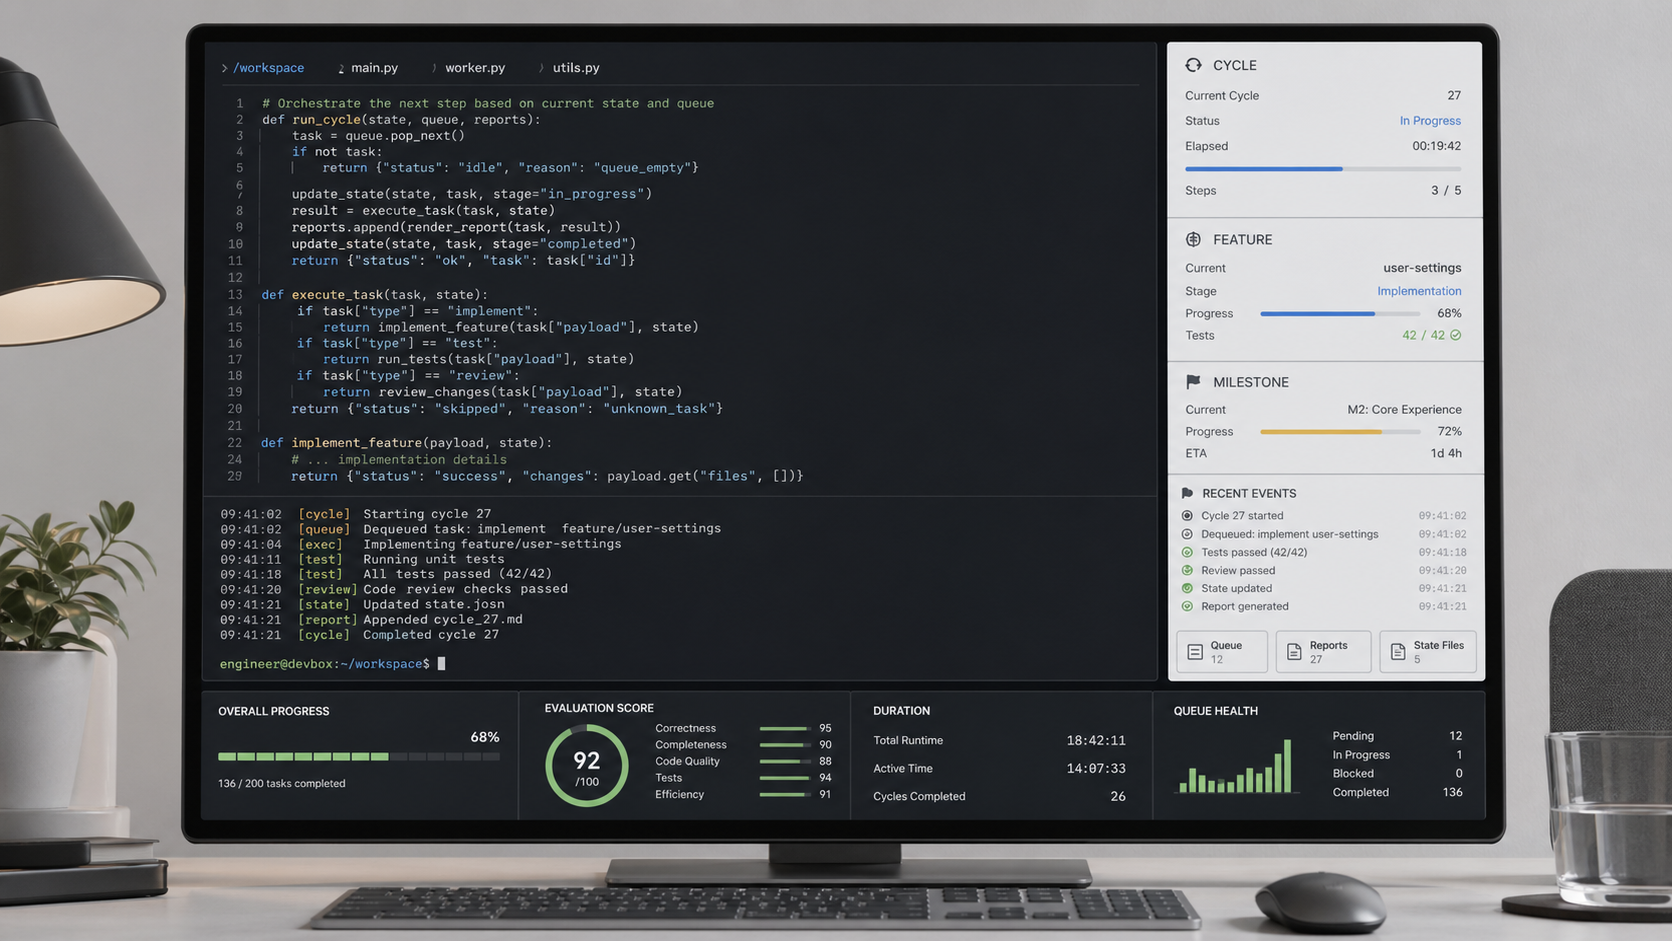
\includegraphics[width=\linewidth,height=0.64\textheight,keepaspectratio]{assets/opencode-observability.png}
    \column{0.40\textwidth}
    \begin{block}{Sidebar}
      Cycle、Feature Queue、当前 Milestone、最近事件。
    \end{block}
    \begin{block}{Footer}
      当前 step、进度、score、heartbeat、duration / token / cost。
    \end{block}
    \begin{alertblock}{判断}
      状态面板不应该成为第二套状态系统，它只应投影 \texttt{.pipeline/}。
    \end{alertblock}
  \end{columns}
\end{frame}

\section{命令面与使用方式}
\WorkflowSectionFrame{Part IV}{按命令解释系统为什么存在}{assets/opencode-observability.png}

\begin{frame}{为什么用命令来组织，而不是只列 Feature}
  \begin{block}{设计判断}
    Feature 适合描述“系统有什么能力”，命令适合描述“用户什么时候该怎么用”。Slides 面向演示时，命令面比 Feature Map 更接近真实使用路径。
  \end{block}
  \begin{columns}[T,totalwidth=\textwidth]
    \column{0.31\textwidth}
    \begin{block}{入口}
      初始化、计划、澄清、拆解。
    \end{block}
    \column{0.31\textwidth}
    \begin{block}{执行}
      开始、恢复、暂停、跳过、状态。
    \end{block}
    \column{0.31\textwidth}
    \begin{block}{收尾}
      修补、审计、报告、展示、发布。
    \end{block}
  \end{columns}
\end{frame}

\begin{frame}{命令枚举 1：初始化与计划}
  \scriptsize
  \begin{tabularx}{\textwidth}{p{0.24\linewidth}p{0.32\linewidth}X}
    \toprule
    命令 & 怎么用 & 为什么需要 \\
    \midrule
    \CommandRow{/hw:init}{初始化或重扫项目，生成架构感知上下文。}{让 Agent 先知道项目形状，再开始计划。}
    \CommandRow{/hw:guide}{不知道从哪开始时走交互式引导。}{降低新项目接入成本。}
    \CommandRow{/hw:plan}{进入 Discover / Decompose / Generate / Confirm。}{把需求先变成可审查计划。}
    \CommandRow{/hw:plan --batch}{一次规划多个 Feature。}{解决长规划中反复开计划流程的问题。}
    \CommandRow{/hw:plan --insert}{用自然语言调整 Feature Queue。}{允许中途插队，但保留队列审计。}
    \bottomrule
  \end{tabularx}
\end{frame}

\begin{frame}{命令枚举 2：计划维护与规则}
  \scriptsize
  \begin{tabularx}{\textwidth}{p{0.24\linewidth}p{0.32\linewidth}X}
    \toprule
    命令 & 怎么用 & 为什么需要 \\
    \midrule
    \CommandRow{/hw:plan:review}{Milestone 完成后检查后续计划是否受影响。}{防止前一段实现改变架构，后一段还按旧假设执行。}
    \CommandRow{/hw:plan:extend}{给活跃 Cycle 追加 Milestone。}{处理遗留问题或新增范围，不必重开一整轮。}
    \CommandRow{/hw:rules}{调整规则严重级、自然语言规则和规则包。}{把反复提醒沉淀成长期约束。}
    \CommandRow{/hw:compact}{生成大型状态文件的 compact view。}{让 Agent 在大上下文项目里仍能快速读准事实。}
    \bottomrule
  \end{tabularx}
\end{frame}

\begin{frame}{命令枚举 3：执行与恢复}
  \scriptsize
  \begin{tabularx}{\textwidth}{p{0.22\linewidth}p{0.34\linewidth}X}
    \toprule
    命令 & 怎么用 & 为什么需要 \\
    \midrule
    \CommandRow{/hw:start}{从当前计划开始执行。}{进入 Milestone 流程，把计划变成实际变更。}
    \CommandRow{/hw:resume}{从保存状态恢复。}{中断后不靠模型回忆，而靠 \texttt{.pipeline/}。}
    \CommandRow{/hw:status}{只读查看当前进度。}{不改变状态地了解现在卡在哪里。}
    \CommandRow{/hw:stop}{优雅暂停并留下恢复信息。}{让中断成为可恢复路径。}
    \CommandRow{/hw:skip}{显式跳过当前步骤。}{保留用户决策，避免 Agent 私自越过问题。}
    \bottomrule
  \end{tabularx}
\end{frame}

\begin{frame}{命令枚举 4：轻量讨论、修补与诊断}
  \scriptsize
  \begin{tabularx}{\textwidth}{p{0.22\linewidth}p{0.34\linewidth}X}
    \toprule
    命令 & 怎么用 & 为什么需要 \\
    \midrule
    \CommandRow{/hw:chat}{追加讨论、小范围解释、小修订记录。}{不为每次轻量讨论开新 Milestone，但仍然可落盘。}
    \CommandRow{/hw:patch}{创建、列出或修复旁路 Patch。}{处理不值得开 Milestone 的小问题。}
    \CommandRow{/hw:debug}{从具体现象出发查根因。}{区别于全面审计，直接解决当前失败。}
    \CommandRow{/hw:audit}{做预防性代码审查。}{在发布或大改后主动找风险。}
    \bottomrule
  \end{tabularx}
\end{frame}

\begin{frame}{命令枚举 5：证据、展示与发布}
  \scriptsize
  \begin{tabularx}{\textwidth}{p{0.22\linewidth}p{0.34\linewidth}X}
    \toprule
    命令 & 怎么用 & 为什么需要 \\
    \midrule
    \CommandRow{/hw:check}{快速检查 config、state、prompts、rules。}{发布前先确认工作区健康。}
    \CommandRow{/hw:log}{读取统一生命周期日志。}{让历史不只存在于聊天记录。}
    \CommandRow{/hw:report}{查看最近 Milestone 或 Cycle 报告。}{把结果和验证结论显式化。}
    \CommandRow{/hw:showcase}{生成介绍文档、技术报告、Slides、Poster。}{把工程成果转成可展示材料。}
    \CommandRow{/hw:release}{跑回归、版本、changelog 和发布流程。}{把交付收束成可复现的 release。}
    \bottomrule
  \end{tabularx}
\end{frame}

\begin{frame}{Feature Queue：长规划的中层调度器}
  \begin{itemize}
    \item \texttt{/hw:plan --batch}：一次 Discover 覆盖多个 Feature。
    \item upfront / just-in-time decomposition：先排队，再按需要拆 Milestone。
    \item \texttt{/hw:plan --insert}：自然语言 queue edit。
    \item auto-chain + \texttt{gate: confirm}：能连续推进，也能在关键点停下。
    \item Feature Queue 与 metrics 分离：队列负责顺序，指标负责证据。
  \end{itemize}
  \vspace{0.25cm}
  \begin{block}{核心价值}
    把“每个功能重新走一遍完整计划流程”压缩成“先统一 Discover，再按顺序推进执行”。
  \end{block}
\end{frame}

\begin{frame}{Progressive Discover 与 Test Profiles}
  \begin{columns}[T,totalwidth=\textwidth]
    \column{0.48\textwidth}
    \begin{block}{Progressive Discover}
      先问任务类别、目标效果和验证方式，再进入假设、歧义、权衡和验收标准。它解决的是“还没搞清楚就急着拆 Milestone”的问题。
    \end{block}
    \column{0.48\textwidth}
    \begin{block}{Test Profiles}
      webapp 必须有浏览器证据，agent-service 必须有 CLI 场景，research 必须有 baseline / script / delta。它解决的是“计划阶段没定义怎么验收”的问题。
    \end{block}
  \end{columns}
\end{frame}

\begin{frame}{README、Skills 与分发维护}
  \begin{columns}[T,totalwidth=\textwidth]
    \column{0.48\textwidth}
    \begin{block}{README automation}
      \texttt{templates/readme-spec.md}、managed blocks、\texttt{update\_readme}、\texttt{readme-freshness} 让 README 跟随真实命令面更新。
    \end{block}
    \column{0.48\textwidth}
    \begin{block}{Skill governance}
      \texttt{references/skill-spec.md} 和 \texttt{skill-quality} 把 Codex、Claude Code、OpenCode 的 skill/command 映射纳入可检查合同。
    \end{block}
  \end{columns}
\end{frame}

\section{Demo / Evaluation / Discussion}
\WorkflowSectionFrame{Part V}{演示路径、验证闭环与未来问题}{assets/opencode-observability.png}

\begin{frame}{Demo Route}
  \begin{enumerate}
    \item \texttt{/hw:init} 或 \texttt{/hw:guide}：让系统理解项目。
    \item \texttt{/hw:plan --batch}：用 Progressive Discover 形成 Feature Queue。
    \item \texttt{/hw:start}：执行第一个 Milestone。
    \item \texttt{/hw:chat}：记录轻量追加讨论。
    \item \texttt{/hw:patch}：旁路修复展示问题。
    \item \texttt{/hw:status} / OpenCode panels：查看状态投影。
    \item \texttt{/hw:release}：以 tests、reports、PDF 和 tag 收尾。
  \end{enumerate}
\end{frame}

\begin{frame}{V9.1 验证证据}
  \small
  \begin{tabularx}{\textwidth}{p{0.24\linewidth}p{0.38\linewidth}X}
    \toprule
    能力 & 自动化验证 & 结果 \\
    \midrule
    README / Feature Queue docs & \texttt{readme-feature-queue.test.js} & pass \\
    Skill governance & \texttt{skill-quality.test.js} + \texttt{checkSkillQuality()} & pass \\
    OpenCode panels & \texttt{opencode-status.test.js} + \texttt{opencode-panels.test.js} & pass \\
    Batch Planning & \texttt{batch-plan.test.js} + \texttt{feature-queue-ops.test.js} & pass \\
    Chat / Discover / Profiles & 对应核心测试集 & pass \\
    Final regression & \texttt{node --test core/test/*.test.js} + \texttt{python3 tests/run\_regression.py} & 75/75 + 60/60 \\
    \bottomrule
  \end{tabularx}
\end{frame}

\begin{frame}{和其他工具的关系}
  \small
  \begin{tabularx}{\textwidth}{lXXXX}
    \toprule
    Tool & Repo visibility & Planning & Recoverability & Validation \\
    \midrule
    Web GPT / Gemini & 弱 & 弱 & 弱 & 弱 \\
    Copilot & 中 & 弱 & 弱 & 弱 \\
    AntiGravity & 中 & 中下 & 弱 & 弱 \\
    Claude Code & 强 & 中上 & 中 & 中 \\
    Superpowers & 强 & 中 & 中 & 中 \\
    Notion AI + Codex & 强 & 强 & 中上 & 中上 \\
    Hypo-Workflow & 强 & 强 & 强 & 强 \\
    \bottomrule
  \end{tabularx}
  \vspace{0.25cm}
  \begin{alertblock}{技术性评价}
    我想解决的不是“哪个模型更聪明”，而是“哪个系统能稳定承载长期工程约束”。
  \end{alertblock}
\end{frame}

\begin{frame}{局限性}
  \begin{itemize}
    \item 仍依赖宿主 Agent 的基础能力，不能替代模型本体。
    \item token / cost 观测仍是 best-effort。
    \item OpenCode 状态面板以观测为主，不直接调度。
    \item Test Profile runtime 在本仓库主要体现为 evidence contract。
    \item 当前多 Agent / 多模型路由仍是下一轮计划项，不是 V9.1 已完成能力。
  \end{itemize}
\end{frame}

\begin{frame}{未来工作}
  \begin{itemize}
    \item pure analysis assistant mode
    \item workflow generalization beyond code writing
    \item richer observability and metrics
    \item stronger cross-platform adapters and shared standards
    \item 探讨 Harness 能否降低对模型工程智力的需求：把更多规划、压缩、验证和恢复能力外置，减少“必须用最强模型才能稳住工程”的依赖。
  \end{itemize}
\end{frame}

\begin{frame}{结论}
  \begin{block}{结论}
    对复杂 AI Coding，真正决定质量上限的通常不是单次模型回答，而是外部工程约束系统是否完备。
  \end{block}
  \vspace{0.6cm}
  \centering
  {\Large\bfseries\color{WorkflowBlue}Hypo-Workflow 的工作，是把这些约束从聊天窗口搬进工程系统。}
\end{frame}

\end{document}
